\documentclass{book}
\usepackage[a4paper,top=2.5cm,bottom=2.5cm,left=2.5cm,right=2.5cm]{geometry}
\usepackage{makeidx}
\usepackage{natbib}
\usepackage{graphicx}
\usepackage{multicol}
\usepackage{float}
\usepackage{listings}
\usepackage{color}
\usepackage{ifthen}
\usepackage[table]{xcolor}
\usepackage{textcomp}
\usepackage{alltt}
\usepackage{ifpdf}
\ifpdf
\usepackage[pdftex,
            pagebackref=true,
            colorlinks=true,
            linkcolor=blue,
            unicode
           ]{hyperref}
\else
\usepackage[ps2pdf,
            pagebackref=true,
            colorlinks=true,
            linkcolor=blue,
            unicode
           ]{hyperref}
\usepackage{pspicture}
\fi
\usepackage[utf8]{inputenc}
\usepackage{mathptmx}
\usepackage[scaled=.90]{helvet}
\usepackage{courier}
\usepackage{sectsty}
\usepackage{amssymb}
\usepackage[titles]{tocloft}
\usepackage{doxygen}
\lstset{language=C++,inputencoding=utf8,basicstyle=\footnotesize,breaklines=true,breakatwhitespace=true,tabsize=4,numbers=left }
\makeindex
\setcounter{tocdepth}{3}
\renewcommand{\footrulewidth}{0.4pt}
\renewcommand{\familydefault}{\sfdefault}
\hfuzz=15pt
\setlength{\emergencystretch}{15pt}
\hbadness=750
\tolerance=750
\begin{document}
\hypersetup{pageanchor=false,citecolor=blue}
\begin{titlepage}
\vspace*{7cm}
\begin{center}
{\Large My Project \\[1ex]\large v2.\-1.\-3 }\\
\vspace*{1cm}
{\large Generated by Doxygen 1.8.3.1}\\
\vspace*{0.5cm}
{\small Sun Jan 27 2013 09:12:36}\\
\end{center}
\end{titlepage}
\clearemptydoublepage
\pagenumbering{roman}
\tableofcontents
\clearemptydoublepage
\pagenumbering{arabic}
\hypersetup{pageanchor=true,citecolor=blue}
\chapter{Namespace Index}
\section{Namespace List}
Here is a list of all namespaces with brief descriptions\-:\begin{DoxyCompactList}
\item\contentsline{section}{\hyperlink{namespacemypkg}{mypkg} }{\pageref{namespacemypkg}}{}
\item\contentsline{section}{\hyperlink{namespacemypkg_1_1amod}{mypkg.\-amod} }{\pageref{namespacemypkg_1_1amod}}{}
\end{DoxyCompactList}

\chapter{Hierarchical Index}
\section{Class Hierarchy}
This inheritance list is sorted roughly, but not completely, alphabetically\-:\begin{DoxyCompactList}
\item object\begin{DoxyCompactList}
\item \contentsline{section}{A\-Class}{\pageref{classmypkg_1_1amod_1_1_a_class}}{}
\item \contentsline{section}{My\-Class}{\pageref{classmypkg_1_1_my_class}}{}
\end{DoxyCompactList}
\end{DoxyCompactList}

\chapter{Data Structure Index}
\section{Data Structures}
Here are the data structures with brief descriptions\-:\begin{DoxyCompactList}
\item\contentsline{section}{\hyperlink{classmypkg_1_1amod_1_1_a_class}{A\-Class} }{\pageref{classmypkg_1_1amod_1_1_a_class}}{}
\item\contentsline{section}{\hyperlink{classmypkg_1_1_my_class}{My\-Class} }{\pageref{classmypkg_1_1_my_class}}{}
\end{DoxyCompactList}

\chapter{File Index}
\section{File List}
Here is a list of all files with brief descriptions\-:\begin{DoxyCompactList}
\item\contentsline{section}{mypkg/\hyperlink{____init_____8py}{\-\_\-\-\_\-init\-\_\-\-\_\-.\-py} }{\pageref{____init_____8py}}{}
\item\contentsline{section}{mypkg/\hyperlink{amod_8py}{amod.\-py} }{\pageref{amod_8py}}{}
\end{DoxyCompactList}

\chapter{Namespace Documentation}
\hypertarget{namespacemypkg}{\section{mypkg Namespace Reference}
\label{namespacemypkg}\index{mypkg@{mypkg}}
}
\subsection*{Namespaces}
\begin{DoxyCompactItemize}
\item 
namespace \hyperlink{namespacemypkg_1_1amod}{amod}
\end{DoxyCompactItemize}
\subsection*{Data Structures}
\begin{DoxyCompactItemize}
\item 
class \hyperlink{classmypkg_1_1_my_class}{My\-Class}
\end{DoxyCompactItemize}
\subsection*{Functions}
\begin{DoxyCompactItemize}
\item 
def \hyperlink{namespacemypkg_adc32c158c8d739df6880b458ec5dd8fc}{afunc}
\end{DoxyCompactItemize}


\subsection{Detailed Description}
\begin{DoxyVerb}@package mypkg
This is the primary module of the MyPkg package.

And yet more.
\end{DoxyVerb}
 

\subsection{Function Documentation}
\hypertarget{namespacemypkg_adc32c158c8d739df6880b458ec5dd8fc}{\index{mypkg@{mypkg}!afunc@{afunc}}
\index{afunc@{afunc}!mypkg@{mypkg}}
\subsubsection[{afunc}]{\setlength{\rightskip}{0pt plus 5cm}def mypkg.\-afunc (
\begin{DoxyParamCaption}
{}
\end{DoxyParamCaption}
)}}\label{namespacemypkg_adc32c158c8d739df6880b458ec5dd8fc}
\begin{DoxyVerb}The afunc function takes some parameters and returns a value.\end{DoxyVerb}
 
\hypertarget{namespacemypkg_1_1amod}{\section{mypkg.\-amod Namespace Reference}
\label{namespacemypkg_1_1amod}\index{mypkg.\-amod@{mypkg.\-amod}}
}
\subsection*{Data Structures}
\begin{DoxyCompactItemize}
\item 
class \hyperlink{classmypkg_1_1amod_1_1_a_class}{A\-Class}
\end{DoxyCompactItemize}
\subsection*{Functions}
\begin{DoxyCompactItemize}
\item 
def \hyperlink{namespacemypkg_1_1amod_aeca1bbdf88c36f27ab8c65e01ec5295c}{b\-\_\-func}
\end{DoxyCompactItemize}


\subsection{Function Documentation}
\hypertarget{namespacemypkg_1_1amod_aeca1bbdf88c36f27ab8c65e01ec5295c}{\index{mypkg\-::amod@{mypkg\-::amod}!b\-\_\-func@{b\-\_\-func}}
\index{b\-\_\-func@{b\-\_\-func}!mypkg::amod@{mypkg\-::amod}}
\subsubsection[{b\-\_\-func}]{\setlength{\rightskip}{0pt plus 5cm}def mypkg.\-amod.\-b\-\_\-func (
\begin{DoxyParamCaption}
\item[{}]{a}
\end{DoxyParamCaption}
)}}\label{namespacemypkg_1_1amod_aeca1bbdf88c36f27ab8c65e01ec5295c}

\chapter{Data Structure Documentation}
\hypertarget{classmypkg_1_1amod_1_1_a_class}{\section{A\-Class Class Reference}
\label{classmypkg_1_1amod_1_1_a_class}\index{A\-Class@{A\-Class}}
}
Inheritance diagram for A\-Class\-:\begin{figure}[H]
\begin{center}
\leavevmode
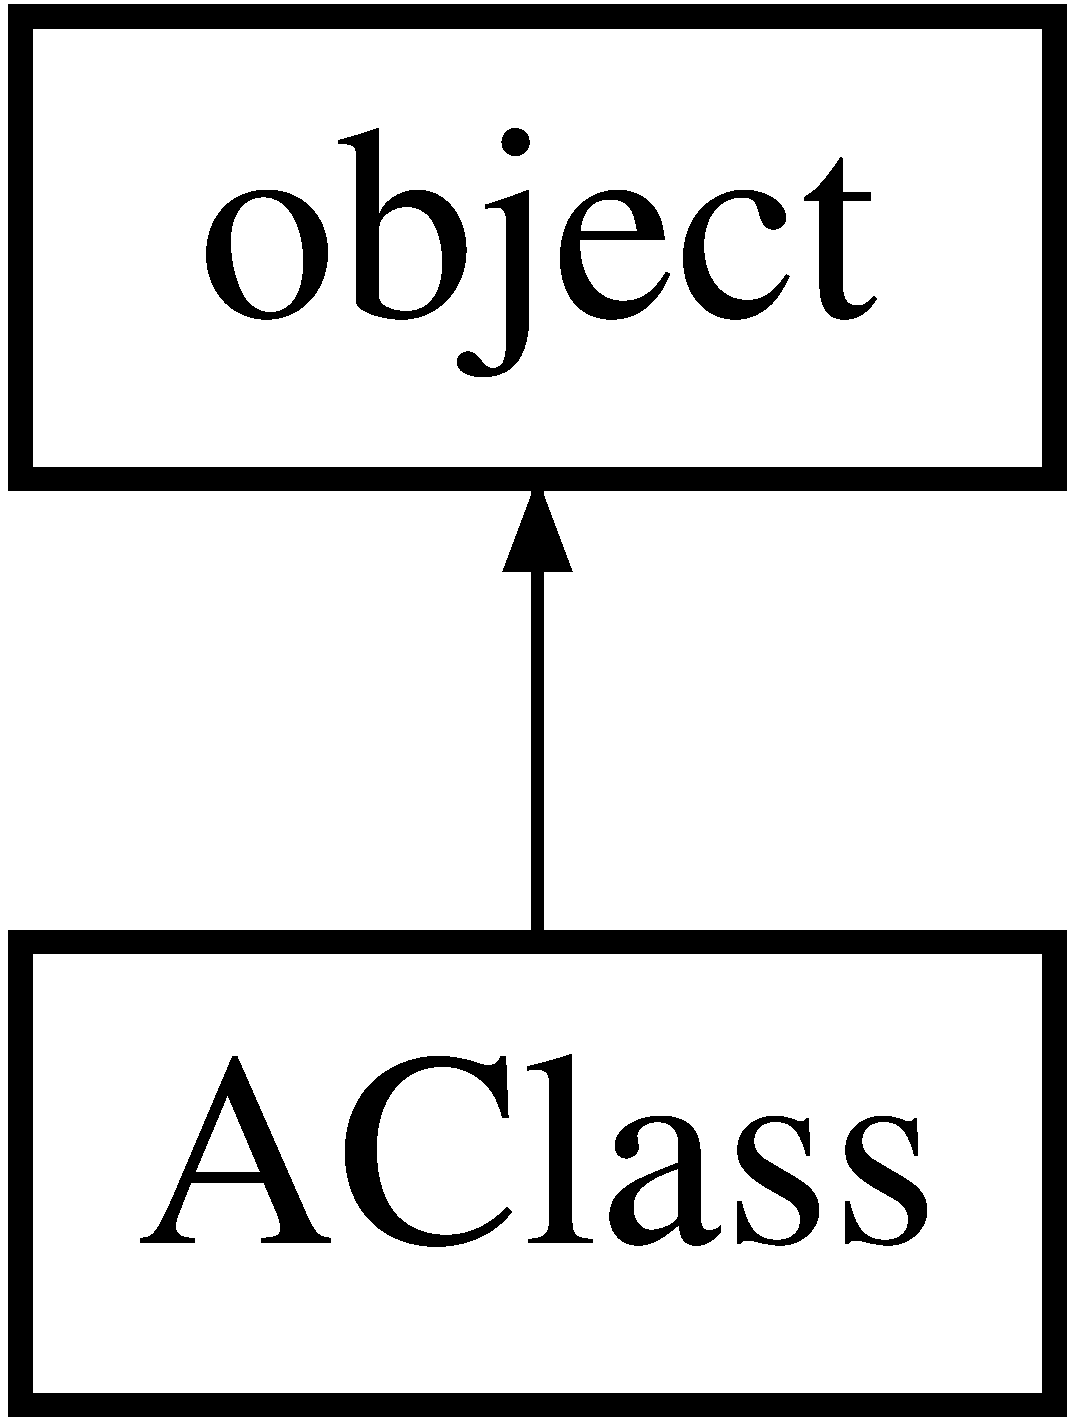
\includegraphics[height=2.000000cm]{classmypkg_1_1amod_1_1_a_class}
\end{center}
\end{figure}
\subsection*{Public Member Functions}
\begin{DoxyCompactItemize}
\item 
def \hyperlink{classmypkg_1_1amod_1_1_a_class_ac775ee34451fdfa742b318538164070e}{\-\_\-\-\_\-init\-\_\-\-\_\-}
\item 
def \hyperlink{classmypkg_1_1amod_1_1_a_class_a821a4d6c0aefe24d7855cedff2cdf1fa}{get\-\_\-age}
\end{DoxyCompactItemize}
\subsection*{Data Fields}
\begin{DoxyCompactItemize}
\item 
\hyperlink{classmypkg_1_1amod_1_1_a_class_ab74e6bf80237ddc4109968cedc58c151}{name}
\end{DoxyCompactItemize}


\subsection{Constructor \& Destructor Documentation}
\hypertarget{classmypkg_1_1amod_1_1_a_class_ac775ee34451fdfa742b318538164070e}{\index{mypkg\-::amod\-::\-A\-Class@{mypkg\-::amod\-::\-A\-Class}!\-\_\-\-\_\-init\-\_\-\-\_\-@{\-\_\-\-\_\-init\-\_\-\-\_\-}}
\index{\-\_\-\-\_\-init\-\_\-\-\_\-@{\-\_\-\-\_\-init\-\_\-\-\_\-}!mypkg::amod::AClass@{mypkg\-::amod\-::\-A\-Class}}
\subsubsection[{\-\_\-\-\_\-init\-\_\-\-\_\-}]{\setlength{\rightskip}{0pt plus 5cm}def \-\_\-\-\_\-init\-\_\-\-\_\- (
\begin{DoxyParamCaption}
\item[{}]{self, }
\item[{}]{name}
\end{DoxyParamCaption}
)}}\label{classmypkg_1_1amod_1_1_a_class_ac775ee34451fdfa742b318538164070e}


\subsection{Member Function Documentation}
\hypertarget{classmypkg_1_1amod_1_1_a_class_a821a4d6c0aefe24d7855cedff2cdf1fa}{\index{mypkg\-::amod\-::\-A\-Class@{mypkg\-::amod\-::\-A\-Class}!get\-\_\-age@{get\-\_\-age}}
\index{get\-\_\-age@{get\-\_\-age}!mypkg::amod::AClass@{mypkg\-::amod\-::\-A\-Class}}
\subsubsection[{get\-\_\-age}]{\setlength{\rightskip}{0pt plus 5cm}def get\-\_\-age (
\begin{DoxyParamCaption}
\item[{}]{self}
\end{DoxyParamCaption}
)}}\label{classmypkg_1_1amod_1_1_a_class_a821a4d6c0aefe24d7855cedff2cdf1fa}


\subsection{Field Documentation}
\hypertarget{classmypkg_1_1amod_1_1_a_class_ab74e6bf80237ddc4109968cedc58c151}{\index{mypkg\-::amod\-::\-A\-Class@{mypkg\-::amod\-::\-A\-Class}!name@{name}}
\index{name@{name}!mypkg::amod::AClass@{mypkg\-::amod\-::\-A\-Class}}
\subsubsection[{name}]{\setlength{\rightskip}{0pt plus 5cm}name}}\label{classmypkg_1_1amod_1_1_a_class_ab74e6bf80237ddc4109968cedc58c151}


The documentation for this class was generated from the following file\-:\begin{DoxyCompactItemize}
\item 
mypkg/\hyperlink{amod_8py}{amod.\-py}\end{DoxyCompactItemize}

\hypertarget{classmypkg_1_1_my_class}{\section{My\-Class Class Reference}
\label{classmypkg_1_1_my_class}\index{My\-Class@{My\-Class}}
}
Inheritance diagram for My\-Class\-:\begin{figure}[H]
\begin{center}
\leavevmode
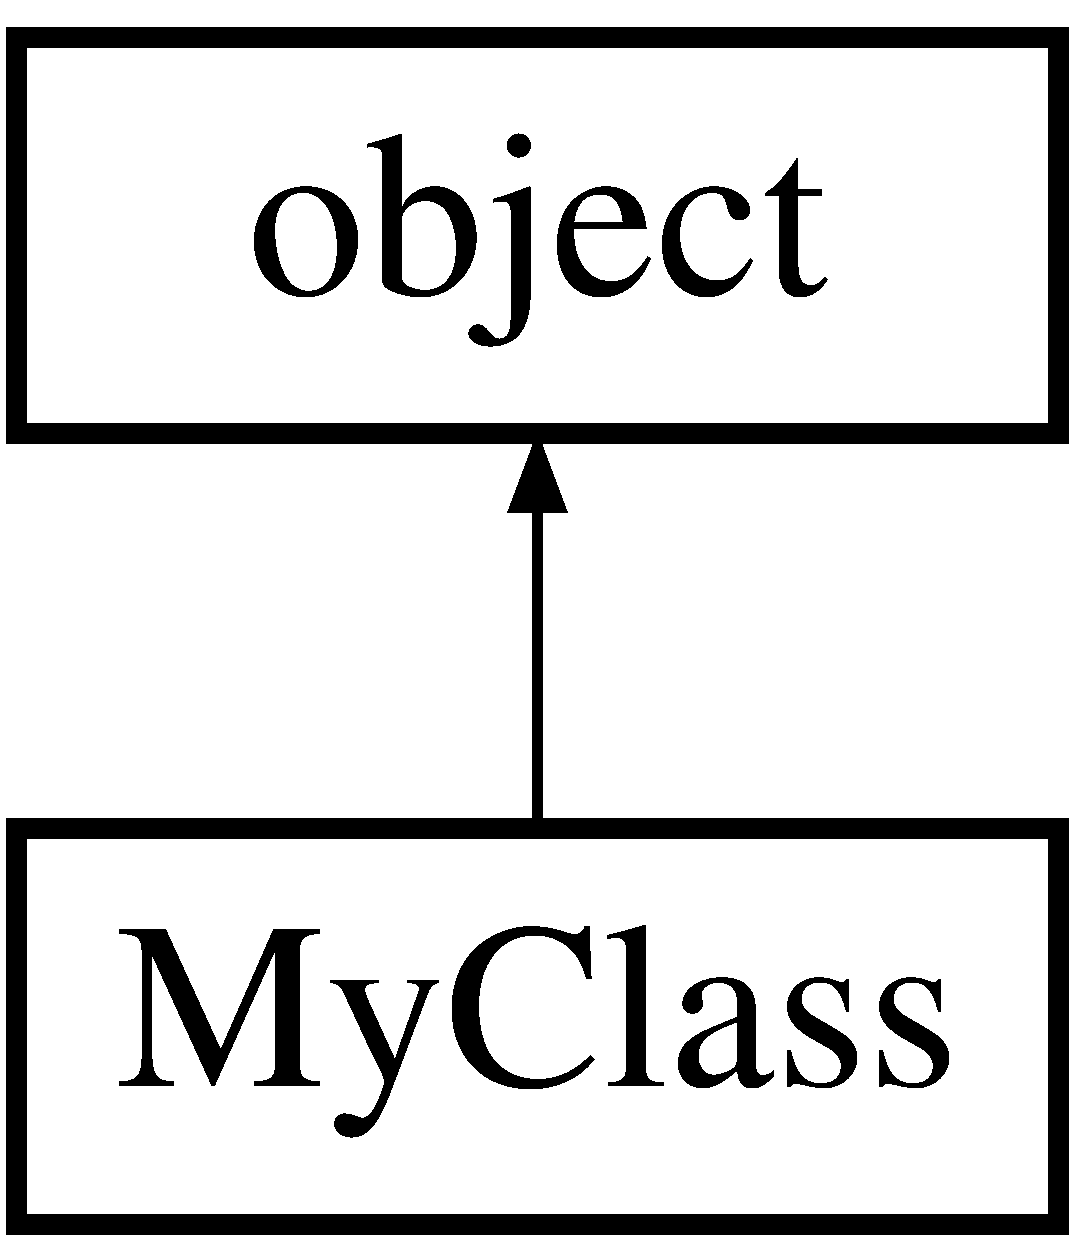
\includegraphics[height=2.000000cm]{classmypkg_1_1_my_class}
\end{center}
\end{figure}
\subsection*{Public Member Functions}
\begin{DoxyCompactItemize}
\item 
def \hyperlink{classmypkg_1_1_my_class_ac775ee34451fdfa742b318538164070e}{\-\_\-\-\_\-init\-\_\-\-\_\-}
\item 
def \hyperlink{classmypkg_1_1_my_class_a2f3160d6b4e517398ca3f9e51b260bb7}{get\-\_\-name}
\end{DoxyCompactItemize}
\subsection*{Data Fields}
\begin{DoxyCompactItemize}
\item 
\hyperlink{classmypkg_1_1_my_class_ab74e6bf80237ddc4109968cedc58c151}{name}
\item 
\hyperlink{classmypkg_1_1_my_class_a9063eb76c0cc024f54d08e4afdf284a3}{ac}
\end{DoxyCompactItemize}


\subsection{Detailed Description}
\begin{DoxyVerb}MyClass represents what my class would look like if it was my child.\end{DoxyVerb}
 

\subsection{Constructor \& Destructor Documentation}
\hypertarget{classmypkg_1_1_my_class_ac775ee34451fdfa742b318538164070e}{\index{mypkg\-::\-My\-Class@{mypkg\-::\-My\-Class}!\-\_\-\-\_\-init\-\_\-\-\_\-@{\-\_\-\-\_\-init\-\_\-\-\_\-}}
\index{\-\_\-\-\_\-init\-\_\-\-\_\-@{\-\_\-\-\_\-init\-\_\-\-\_\-}!mypkg::MyClass@{mypkg\-::\-My\-Class}}
\subsubsection[{\-\_\-\-\_\-init\-\_\-\-\_\-}]{\setlength{\rightskip}{0pt plus 5cm}def \-\_\-\-\_\-init\-\_\-\-\_\- (
\begin{DoxyParamCaption}
\item[{}]{self, }
\item[{}]{name}
\end{DoxyParamCaption}
)}}\label{classmypkg_1_1_my_class_ac775ee34451fdfa742b318538164070e}
\begin{DoxyVerb}Class Constructor.
@param name, A string to be used as the classes name.\end{DoxyVerb}
 

\subsection{Member Function Documentation}
\hypertarget{classmypkg_1_1_my_class_a2f3160d6b4e517398ca3f9e51b260bb7}{\index{mypkg\-::\-My\-Class@{mypkg\-::\-My\-Class}!get\-\_\-name@{get\-\_\-name}}
\index{get\-\_\-name@{get\-\_\-name}!mypkg::MyClass@{mypkg\-::\-My\-Class}}
\subsubsection[{get\-\_\-name}]{\setlength{\rightskip}{0pt plus 5cm}def get\-\_\-name (
\begin{DoxyParamCaption}
\item[{}]{self}
\end{DoxyParamCaption}
)}}\label{classmypkg_1_1_my_class_a2f3160d6b4e517398ca3f9e51b260bb7}


\subsection{Field Documentation}
\hypertarget{classmypkg_1_1_my_class_a9063eb76c0cc024f54d08e4afdf284a3}{\index{mypkg\-::\-My\-Class@{mypkg\-::\-My\-Class}!ac@{ac}}
\index{ac@{ac}!mypkg::MyClass@{mypkg\-::\-My\-Class}}
\subsubsection[{ac}]{\setlength{\rightskip}{0pt plus 5cm}ac}}\label{classmypkg_1_1_my_class_a9063eb76c0cc024f54d08e4afdf284a3}
\hypertarget{classmypkg_1_1_my_class_ab74e6bf80237ddc4109968cedc58c151}{\index{mypkg\-::\-My\-Class@{mypkg\-::\-My\-Class}!name@{name}}
\index{name@{name}!mypkg::MyClass@{mypkg\-::\-My\-Class}}
\subsubsection[{name}]{\setlength{\rightskip}{0pt plus 5cm}name}}\label{classmypkg_1_1_my_class_ab74e6bf80237ddc4109968cedc58c151}


The documentation for this class was generated from the following file\-:\begin{DoxyCompactItemize}
\item 
mypkg/\hyperlink{____init_____8py}{\-\_\-\-\_\-init\-\_\-\-\_\-.\-py}\end{DoxyCompactItemize}

\chapter{File Documentation}
\hypertarget{____init_____8py}{\section{mypkg/\-\_\-\-\_\-init\-\_\-\-\_\-.py File Reference}
\label{____init_____8py}\index{mypkg/\-\_\-\-\_\-init\-\_\-\-\_\-.\-py@{mypkg/\-\_\-\-\_\-init\-\_\-\-\_\-.\-py}}
}
\subsection*{Data Structures}
\begin{DoxyCompactItemize}
\item 
class \hyperlink{classmypkg_1_1_my_class}{My\-Class}
\end{DoxyCompactItemize}
\subsection*{Namespaces}
\begin{DoxyCompactItemize}
\item 
namespace \hyperlink{namespacemypkg}{mypkg}
\end{DoxyCompactItemize}
\subsection*{Functions}
\begin{DoxyCompactItemize}
\item 
def \hyperlink{namespacemypkg_adc32c158c8d739df6880b458ec5dd8fc}{afunc}
\end{DoxyCompactItemize}

\hypertarget{amod_8py}{\section{mypkg/amod.py File Reference}
\label{amod_8py}\index{mypkg/amod.\-py@{mypkg/amod.\-py}}
}
\subsection*{Data Structures}
\begin{DoxyCompactItemize}
\item 
class \hyperlink{classmypkg_1_1amod_1_1_a_class}{A\-Class}
\end{DoxyCompactItemize}
\subsection*{Namespaces}
\begin{DoxyCompactItemize}
\item 
namespace \hyperlink{namespacemypkg_1_1amod}{mypkg.\-amod}
\end{DoxyCompactItemize}
\subsection*{Functions}
\begin{DoxyCompactItemize}
\item 
def \hyperlink{namespacemypkg_1_1amod_aeca1bbdf88c36f27ab8c65e01ec5295c}{b\-\_\-func}
\end{DoxyCompactItemize}

\addcontentsline{toc}{part}{Index}
\printindex
\end{document}
